\subsection{Operation Model for init}

\label{OM-init}


The \msrcode{init} operation has the following properties:

	\begin{operationmodel}
	\addheading{Operation}
	\adddoublerow{init}{used to create an instance of the actor together with its interface instances and update the assocations with the \msrcode{ctState} instance.}


	\addrowheading{Return type}
	\addsinglerow{ptBoolean}

		


	\end{operationmodel}



	
	
	
	





Figure \ref{fig:lu.uni.lassy.excalibur.examples.icrash-OM-scopeView-operation-scope-actMsrCreator-init}

\begin{figure}[htbp]
\begin{center}

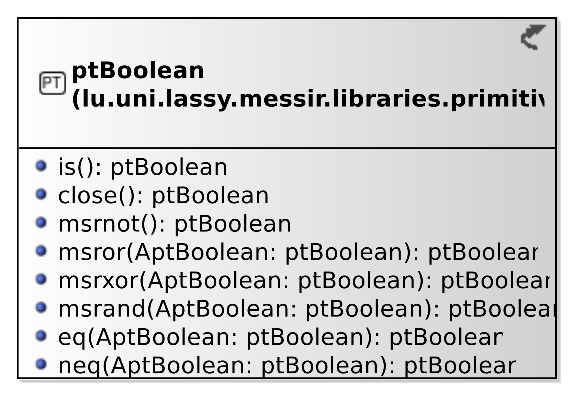
\includegraphics[
angle=0
]{./images-report-gen/operation-model/operation-scope-actMsrCreator-init.eps}
\end{center}
\caption[lu.uni.lassy.excalibur.examples.icrash Operation Scope: operation-scope-actMsrCreator-init]{}
\label{fig:lu.uni.lassy.excalibur.examples.icrash-OM-scopeView-operation-scope-actMsrCreator-init}
\end{figure}
\vspace{0.5cm}

